\begin{center}
	\textbf{Scan History Feedback Questionnaire}\par
	\textbf{Participant No.}\par
\end{center}

\vspace{0.5cm}

\begin{figure}[h]
\begin{center}
	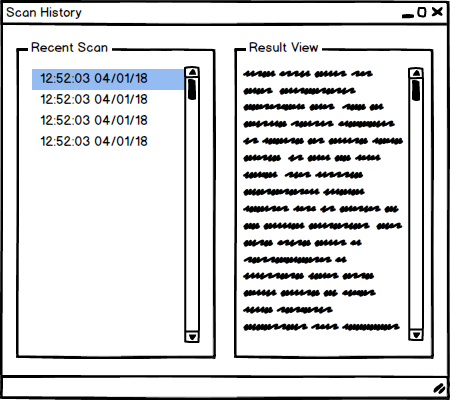
\includegraphics[width=0.75\textwidth]{img/scan_history_mockup.png}
\end{center}
\end{figure}

\vspace{0.5cm}

The above image shows the scan history window, which displays all the users scans based on the time the scan was
performed. Selecting a scan item on the left panel brings up the scan results for that item.

\vspace{0.5cm}

\textbf{1.} On a scale from 1 to 10, how clear would you consider the above interface to be?

\begin{center}
	\begin{table}[h]
	\label{my-label}
	\begin{tabularx}{\textwidth}{XXXXXXXXXX}
	\multicolumn{5}{l}{Unclear} & \multicolumn{5}{r}{Clear} \\
	\centering
	1    & 2    & 3    & 4    & 5    & 6    & 7    & 8    & 9    & 10
	\end{tabularx}
	\end{table}
\end{center}

\textbf{2.} Are there any improvements (additions, changes, removals, etc.) you would make to the current design?

\vspace{5cm}
